\documentclass[10pt,a4paper]{article}
\renewcommand{\familydefault}{\sfdefault}
\usepackage[left=3cm, right=3cm, top=2cm, bottom=2cm, textwidth=15cm]{geometry}
\usepackage[utf8]{inputenc}
\usepackage[T1]{fontenc}
\usepackage[german]{babel}
\usepackage{graphicx}
\usepackage{xfrac}
\usepackage{sectsty}
\usepackage{hyperref}
\sectionfont{\rmfamily\selectfont}
\usepackage{ccicons}

\begin{document}
\thispagestyle{empty}
\pagenumbering{gobble}
\title{Rezeptsammlung\\
	\vspace{1cm}
	{\large Projektarbeit im Rahmen der Ausbildung zur Systemgastronomin}\\
	{\small 1.Berufsschuljahr}
	\vspace{2cm}
}
\author{Lisa Machoi}
\date{\today}
\maketitle
\newpage
\thispagestyle{empty}
\tableofcontents
\setcounter{page}{0}
\pagenumbering{arabic}
%
\newpage
\setcounter{page}{1}
\section{Rohkostsalat mit Apfel}

\textbf{Zutaten für 4 Personen:}
\begin{itemize}
  \item 1x Weißkohlkopf
  \item 4x Karotten
  \item 2x Äpfel
  \item 6EL Olivenöl
  \item 6EL Weißweinessig
  \item 2EL Salz
  \item Pfeffer, Zucker, Kümmel nach Geschmack
\end{itemize}

\textbf{Zubereitung:}
\begin{itemize}
  \item Den Weißkohl teilen und danach in dünne Streifen schneiden.
  \item Wir empfehlen hier die Schnittform Julienne.
  \item Danach die Äpfel und die Karotten schälen.
  \item Den Apfel in Achtel teilen.
  \item Salz und Essig hinzufügen und solange fest kneten, bis der Kohl einen eigenen Saft bildet.
  \item Nun mit Pfeffer, Zucker und den anderen Gewürzen abschmecken.
  \item Danach das Gemisch einige Zeit ziehen lassen und fertig ist der Rohkostsalat.
\end{itemize}

\section{\textsc{Amerikanischer Krautsalat}}

\subsection*{Zutaten:}

\begin{tabular}{p{7.5cm} p{7.5cm}}
	& \\
	\sfrac{1}{2} Weißkohlkopf & 1 Karotte \\
	1 Zwiebel & \sfrac{1}{2}TL Pfeffer \\
	\sfrac{1}{2}TL Salz & 1TL Paprikapulver \\
	2EL Weißweinessig & 1TL Senf \\
	125g Mayonnaise & 65g Zucker \\
	60ml Milch & 60ml Buttermilch \\
	3EL Zitronensaft &
\end{tabular}

\subsection*{Serviervorschlag:}


\includegraphics[width=\textwidth]{img/ph.jpg} \cite{uskrautsalat}

\subsection*{So geht's:}
\begin{tabular}{p{15cm}}
	\\
	Den Weißkohl, die Zwiebel und die Karotte in feine Streifen (Julienne) schneiden.\\
	Das Gemüse in einer großen Schüssel vermengen. Die übrigen Zutaten in einer separaten Schüssel verrühren. Danach die Gemüsemischung mit dem Dressing übergießen.\\
	Den Weißkohlsalat nun abgedeckt, mindestens 8h kalt stellen.\\
	Vor dem Servieren noch einmal durchrühren.
\end{tabular}

\section{\textsc{Schneller Gurkensalat mit saurer Sahne und Dill}}

\subsection*{Zutaten:}

\begin{tabular}{p{7.5cm} p{7.5cm}}
	& \\
	1 Salatgurke & 1 Becher Saure Sahne \\
	1 TL Gehackter Dill & Salz, Pfeffer
\end{tabular}

\subsection*{Serviervorschlag:}


\includegraphics[width=\textwidth]{img/ph.jpg} \cite{gurkensalatdill}

\subsection*{So geht's:}

\begin{tabular}{p{15cm}}
	\\
  Die Gurke in dünne Scheiben schneiden, oder mit einer Küchenreibe reiben.\\
  Zusammen mit der sauren Sahne in eine Schüssel geben.\\
  Mit Salz und Pfeffer abschmecken.\\
  Frisch und gekühlt servieren.
\end{tabular}

\section{\textsc{Gurkensalat}}

\subsection*{Zutaten für 2 Portionen:}

\begin{tabular}{p{7.5cm} p{7.5cm}}
	& \\
	\sfrac{1}{2} Gurke & 2EL Olivenöl \\
	1EL Essig & 1TL Zucker \\
	\multicolumn{2}{l}{Salz, Pfeffer, Dill nach Geschmack}
\end{tabular}

\subsection*{Serviervorschlag:}

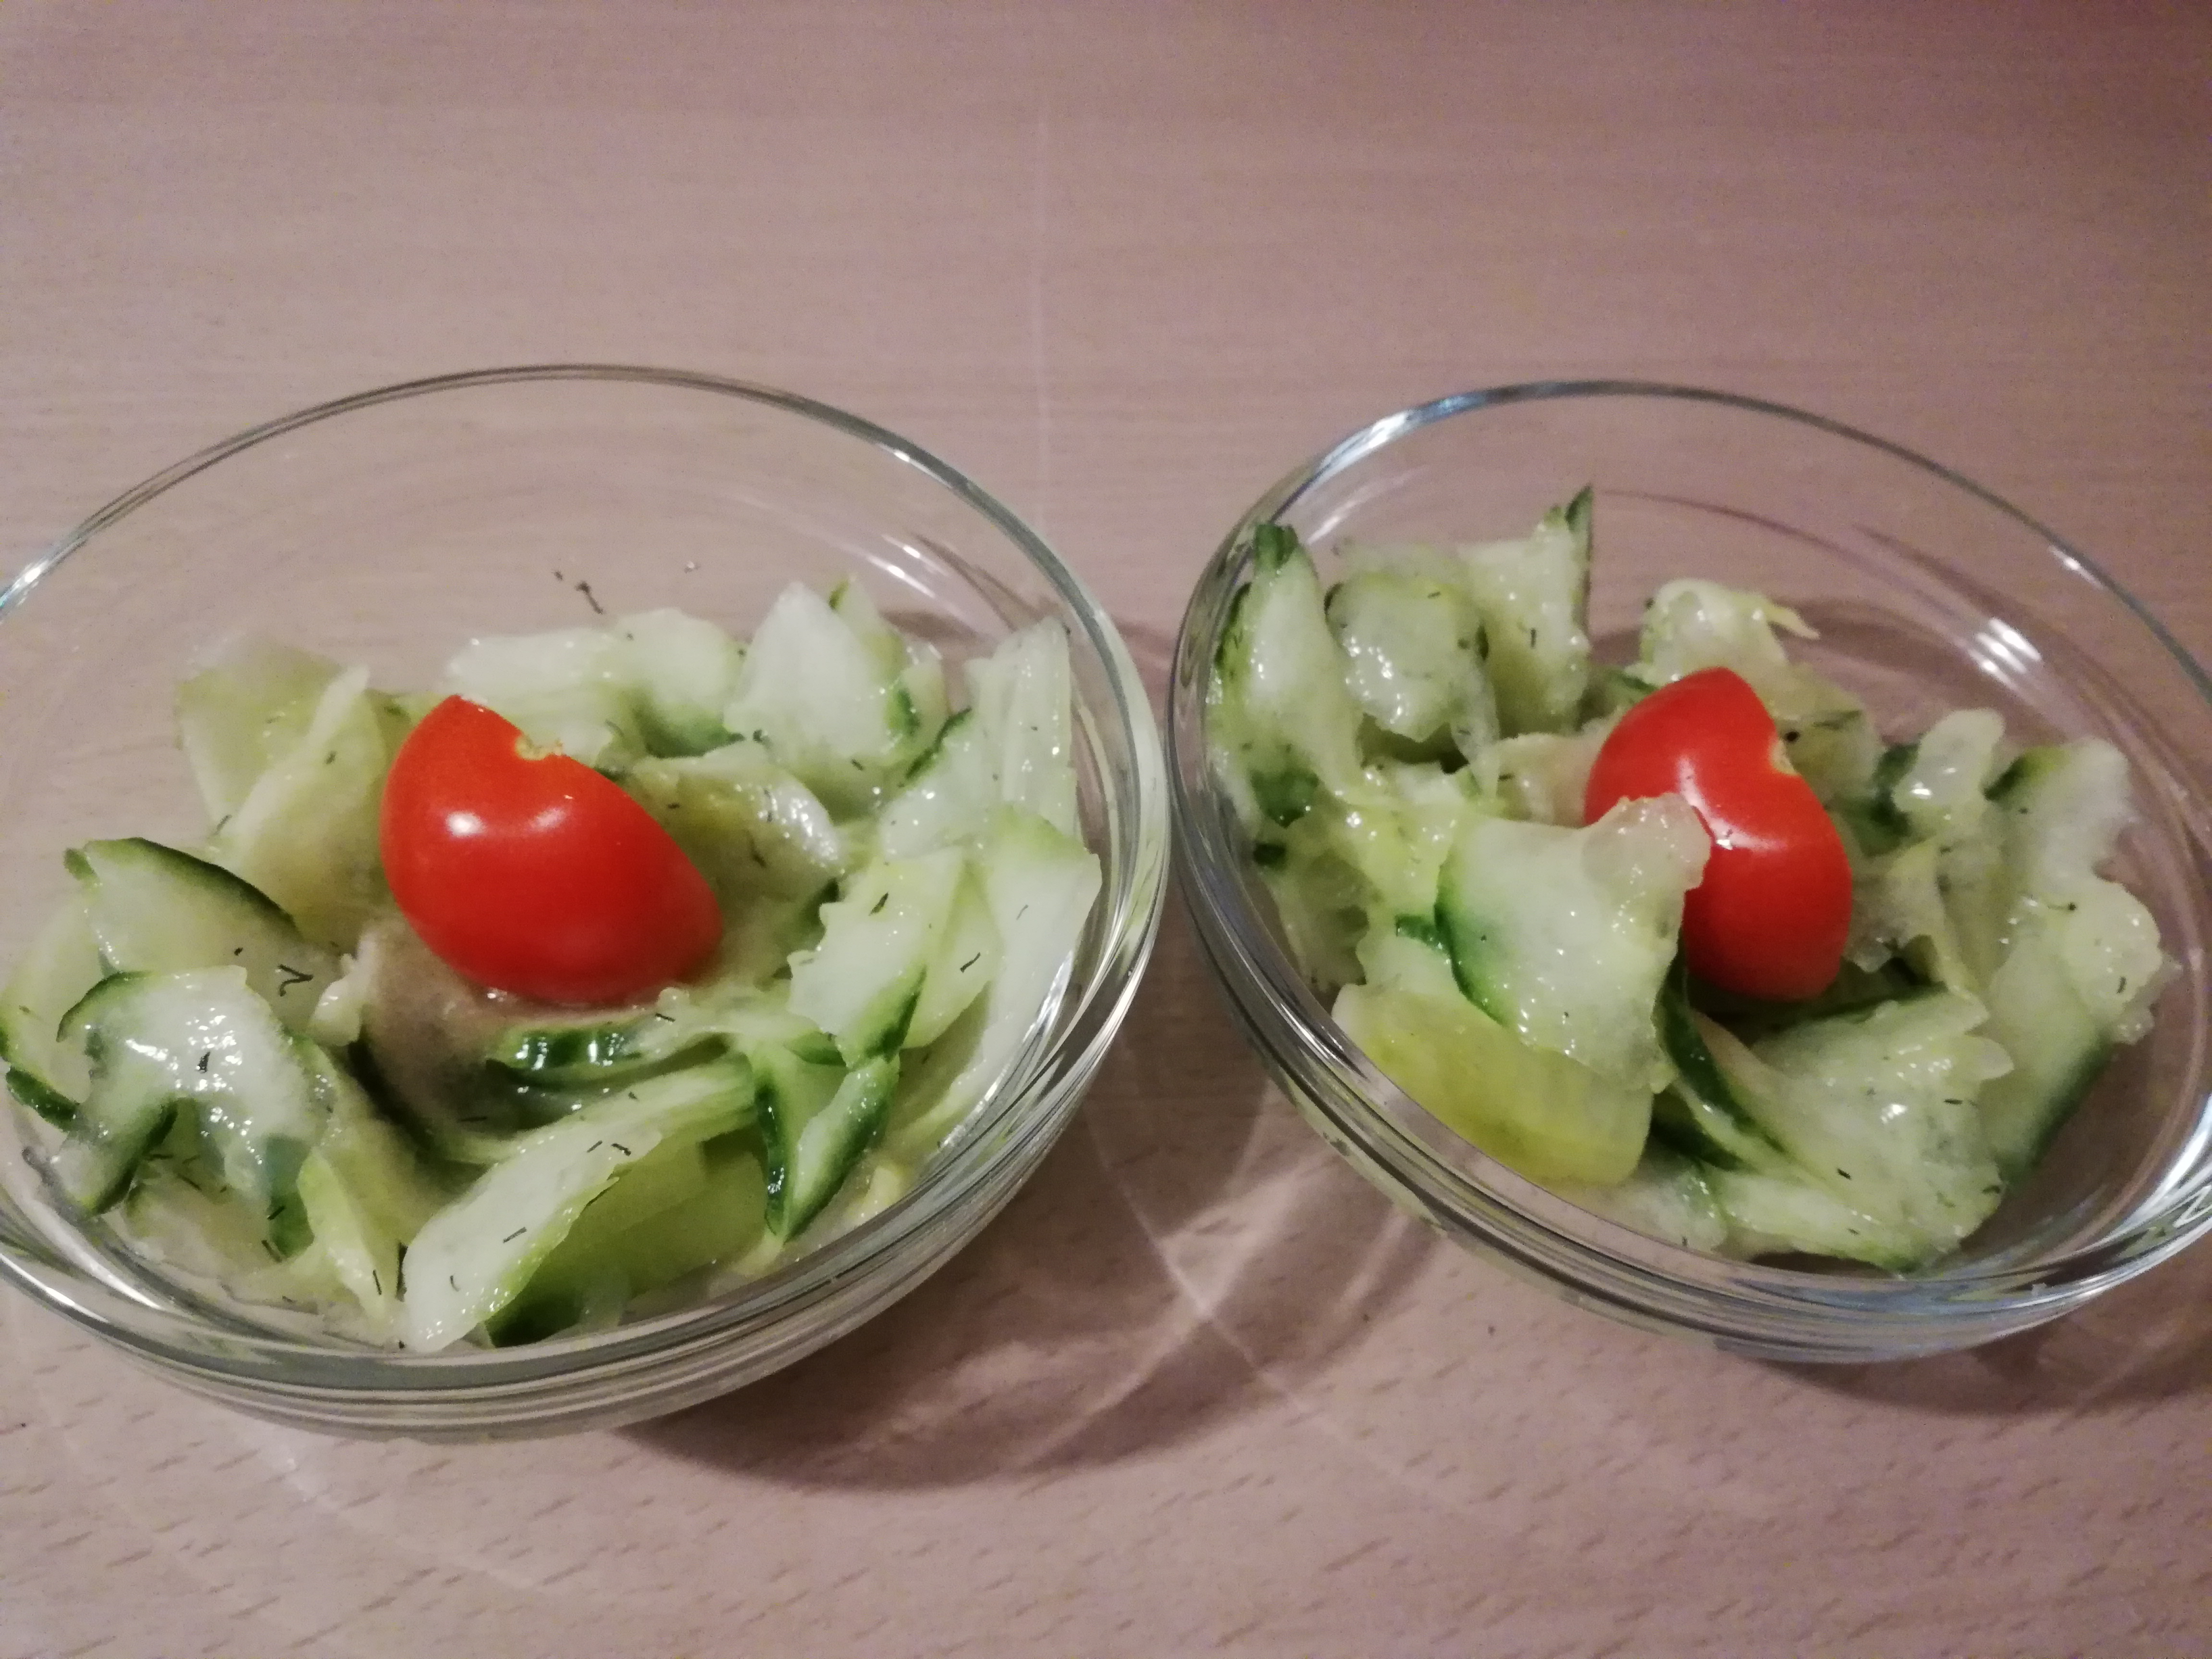
\includegraphics[width=\textwidth]{img/gurkensalat/gurkensalat_fertig.jpg}

\subsection*{So geht's:}

\begin{tabular}{p{15cm}}
	\\
	Die halbe Gurke mit einem Sparschäler teilweise schälen.\\
	So entsteht ein Farbtupfer im fertigen Salat.\\
	Die Gewürze und Öle hinzufügen und alles für etwa 2h ziehen lassen.
\end{tabular}
\section{\textsc{Frühlingshafter Eiersalat}}

\subsection*{Zutaten für 2 Portionen:}

\begin{tabular}{p{7.5cm} p{7.5cm}}
	& \\
	\textbf{Für den Salat:} & \textbf{Für die Soße:} \\
	Verschiedene Blattsalate & 5EL frische Kräuter \\
	1TL Essig & 1 Knoblauchzehe \\
	1EL Olivenöl & 1 Scharlotte \\
	4 hartgekochte Eier & 1TL Senf \\
	Salz und Pfeffer & 3EL Essig \\
	& 4EL Olivenöl \\
\end{tabular}

\subsection*{Serviervorschlag:}


\includegraphics[width=\textwidth]{img/ph.jpg}

\subsection*{So geht's:}

\begin{tabular}{p{15cm}}
	\\
	Eier halbieren und das Eigelb vom Eiweiß trennen. Den Knoblauch und die Schalotten schälen und klein hacken.\\
	Das Eigelb, den Senf, den Knoblauch und die Schalotten in einen Messbecher geben.\\
	Den Essig und das Öl dazugeben und ein paar Minuten ziehen lassen.\\
	In der Zwischenzeit die Kräuter mit einem Wiegemesser fein hacken. Und in zu den anderen Zutaten hinzufügen.\\
	Das Eiweiß ebenfalls klein würfen und mit dazu geben.\\
	Alles fein pürieren und abschmecken.\\
	Die Salate putzen und klein schneiden.\\
	Öl, Essig und Gewürze hinzufügen und 10min ziehen lassen.\\
	In einer großen Schüssel anrichten und mit dem restlichen Ei garnieren.\\
	Baguette oder frische Brötchen dazu servieren.\\
	\textbf{Tipp:}
	Der Salat macht sich super zur Osterzeit. Es bleiben dort öfter mal gekochte Eier übrig, die sich so super verarbeiten lassen.
\end{tabular}

\section{\textsc{Omlett}}

\subsection*{Zutaten:}

\begin{tabular}{p{7.5cm} p{7.5cm}}
	& \\
	6 Eier & 40g Butter \\
	20ml Wasser & 20ml Milch \\
  1TL Salt & Pfeffer, Salz \& Muskat \\
  Schnittlauch zum Garnieren &
\end{tabular}

\subsection*{Serviervorschlag:}


\includegraphics[width=\textwidth]{img/ph.jpg} \cite{omlett}

\subsection*{So geht's:}

\begin{tabular}{p{15cm}}
	\\
  Die Eier aufschlagen und in eine Schüssel geben.\\
  Mit den Gewürzen nach Geschmack würzen und mit Wasser und Milch aufschlagen. \\
  Die Masse in eine heiße Pfanne geben. Nach und nach stocken lassen.\\
  Zusammenklappen und mit Butter bestreichen. 
\end{tabular}

\section{\textsc{Gewienertes Omlett}}

\subsection*{Zutaten für 1 Omlett:}

\begin{tabular}{p{7.5cm} p{7.5cm}}
	& \\
	4 Eier & 2 Wiener Würstchen \\
	\sfrac{1}{2} Zwiebel & 200g Mozzarella \\
	Salz und Pfeffer &
\end{tabular}

\subsection*{Serviervorschlag:}


\includegraphics[width=\textwidth]{img/ph.jpg}

\subsection*{So geht's}

\begin{tabular}{p{15cm}}
	Die Eier in eine Schüssel aufschlagen und schaumig schlagen.\\
	In einer großen Pfanne die Butter schmelzen.\\
	In der Zwischenzeit die Wiener in dünne Scheiben schneiden.\\
	Die Zwiebeln fein würfeln.\\
	Die Eimasse in die Pfanne geben und auf großer Hitze stocken lassen.\\
	Die Wiener und die Zwiebeln auf dem Omlett verteilen.\\
	Mit einem Deckel auf der Pfanne 5min braten.\\
	Auf einem großen Teller servieren.
\end{tabular}

\section{\textsc{Omlett ToMo}}

\subsection*{Zutaten für 1 Omlett:}

\begin{tabular}{p{7.5cm} p{7.5cm}}
	& \\
	4 Eier & 5 Cherrytomaten \\
	2TL Butter & 200g Mozzarella \\
	Salz & Pfeffer \\
	Basilikum nach Geschmack &
\end{tabular}

\subsection*{Serviervorschlag:}


\includegraphics[width=\textwidth]{img/ph.jpg}

\subsection*{So geht's:}

\begin{tabular}{p{15cm}}
	\\
	Die Eier mit einem Schneebesen schaumig schlagen.\\
	Salz und Pfeffer nach Belieben hinzufügen.\\
	Die Butter in einer Pfanne schmelzen lassen.\\
	Die Eimasse in die Pfanne geben und auf großer Hitze stocken lassen.\\
	Den Mozzarella und die Tomaten darauf verteilen.\\
	Mit einem Deckel auf kleiner Flamme 5min braten lassen.\\
	Auf einen großen Teller geben und mit dem Basilikum dekorieren.\\
\end{tabular}

\section{\textsc{Spiegelei}}

\subsection*{Zutaten für 2 Portionen:}

\begin{tabular}{p{7.5cm} p{7.5cm}}
	& \\
	2 Eier & Salz \& Pfeffer \\
	Öl zum Braten & 
\end{tabular}

\subsection*{Serviervorschlag:}

%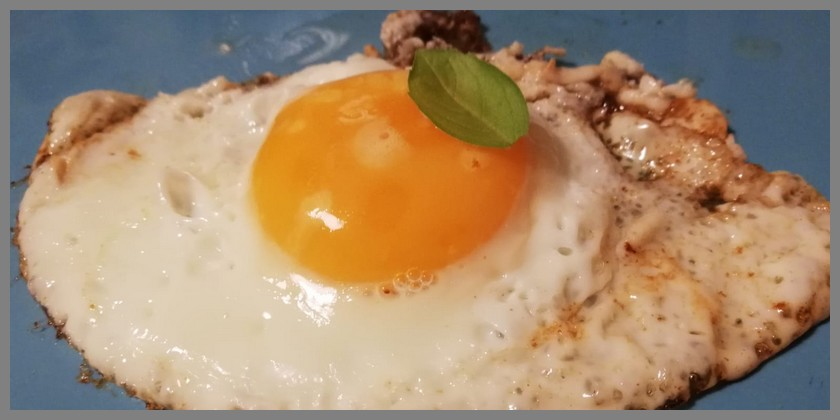
\includegraphics[width=\textwidth]{img/spiegelei.jpg} \cite{spiegelei}

\subsection*{So geht's:}

\begin{tabular}{p{15cm}}
	\\
	Das Öl in einer Pfanne erhitzen.\\
	Ei in das Öl aufschlagen. \\
	Salzen und Deckel auf die Pfanne setzten und je nach Geschmack braten.\\
	Mit einem Pfannenwender das Ei aus der Pfanne nehmen und pfeffern.
\end{tabular}
\section{\textsc{Spiegelei auf italienisch}}

\subsection*{Zutaten für 2 Portionen:}

\begin{tabular}{p{7.5cm} p{7.5cm}}
	& \\
	6 Eier & Mozzarella \\
	Öl zum Braten & Gewürze nach Geschmack
\end{tabular}

\subsection*{Serviervorschlag:}

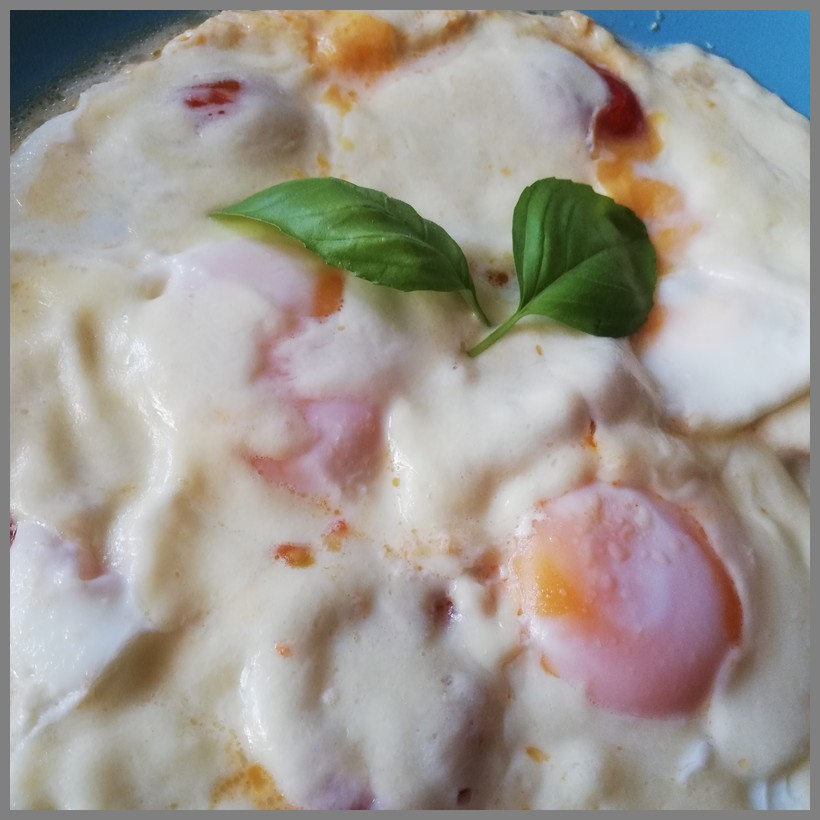
\includegraphics[width=\textwidth]{img/spiegelei_ita.jpg} \cite{itaspiegelei}

\subsection*{So geht's:}

\begin{tabular}{p{15cm}}
	\\
  Öl in der Pfanne erhitzen.\\
  Tomate in dünne Scheiben schneiden und in der Pfanne andünsten.\\
  Nun die Eier in die Pfanne schlagen.\\
  Sobald es anfängt zu stocken, den Mozzarella gleichmäßig darauf verteilen.\\
  Würzen und fertig.
\end{tabular}

\section{\textsc{Rührei}}

\subsection*{Zutaten:}

\begin{tabular}{p{7.5cm} p{7.5cm}}
	& \\
	3 Eier & 125ml Milch \\
	1EL Öl & Salz, Pfeffer, Muskatnuss
\end{tabular}

\subsection*{Serviervorschlag:}

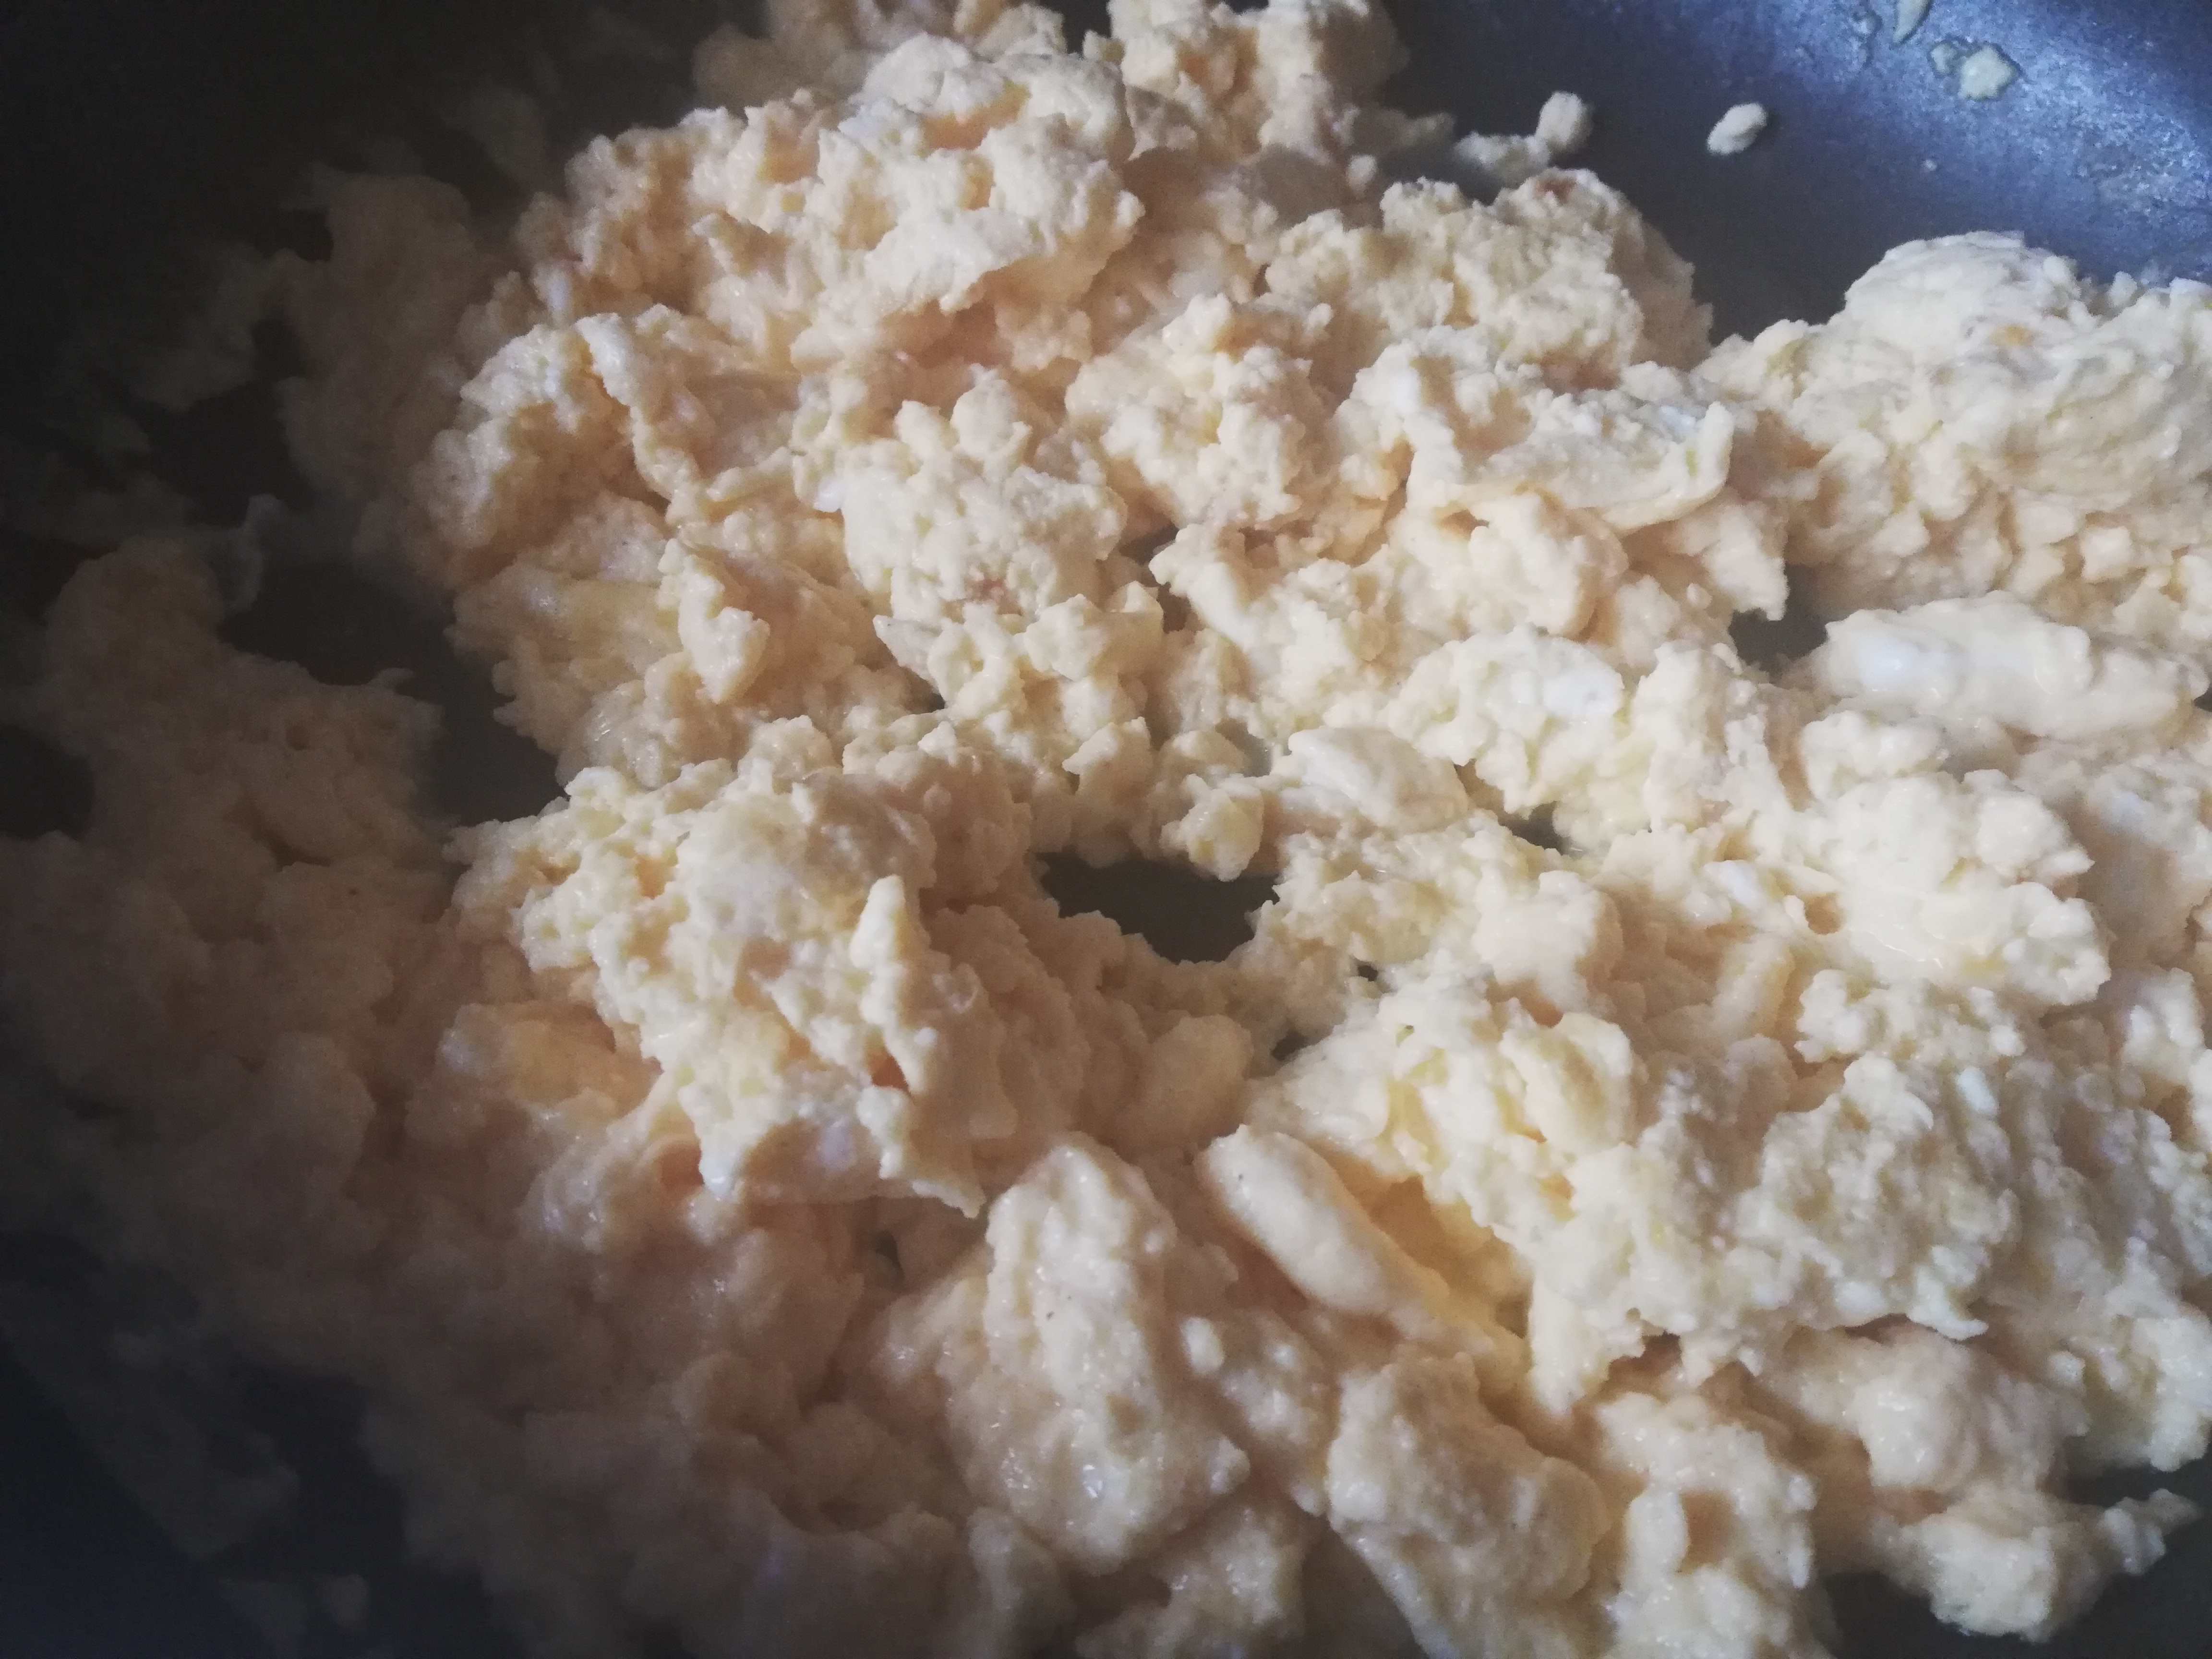
\includegraphics[width=\textwidth]{img/ruehrei/ruehrei_fertig.jpg}

\subsection*{So geht's:}

\begin{tabular}{p{15cm}}
	\\
	Die Milch in einem Messbecher abfüllen. Die Eier auch in diesen schlagen. Mit einem Schneebesen zu einer glatten Masse rühren.\\
	Je nach Geschmack mit Salz, Pfeffer und Muskatnuss würzen.\\
	Öl in einer Pfanne erhitzen. Die gesamte Eimasse hineingeben.\\
	Kurz stocken lassen. Das Ei nun mit einem Pfannenschaber von innen nach außen schieben. Vorgang so lange wiederholen, bis das gesamte Ei gestockt ist.
\end{tabular}
\section{\textsc{Rührei auf Vollkornbrötchen}}

\subsection*{Zutaten:}

\begin{tabular}{p{7.5cm} p{7.5cm}}
	& \\
	5 Eier & 2 Vollkornbrötchen \\
	1 Tomate & 20g Butter \\
  1EL Kresse & 2 Salatblätter \\
  Frische Käuter & Remoulade \\
  Öl zum Braten & Schluck Mineralwasser \\
  Salz, Pfeffer \& Muskatnuss
\end{tabular}

\subsection*{Serviervorschlag:}


\includegraphics[width=\textwidth]{img/ph.jpg}

\subsection*{So geht's:}

\begin{tabular}{p{15cm}}
	\\
  Eier, Kräuter und Mineralwasser in einer Schüssel vermengen.\\
  Öl in einer flachen Pfanne erhitzen.\\
  Die Eimasse hineingeben, tocken lassen und nach und nach mit einem Schaber von außen nach innen schieben.\\
  In der Zwischenzeit die Brötchen aufschneiden und mit Remoulade bestreichen.\\
  Ein Salatblatt darauf platzieren.\\
  Das fertige Rührei auf dem Salat verteilen und mit einer halben Tomate garnieren.
\end{tabular}

\section{\textsc{Französisches Ei im Näpfchen}}

\subsection*{Zutaten für 2 Schälchen:}

\begin{tabular}{p{7.5cm} p{7.5cm}}
	& \\
	6EL Schmand & 2 Eier \\
	2El frische gehackte Käuter & 2 Cocktailtomaten \\
  Salz, Pfeffer \& Muskat & Baquette als Beilage
\end{tabular}

\subsection*{Serviervorschlag:}


\includegraphics[width=\textwidth]{img/ph.jpg}

\subsection*{So geht's:}

\begin{tabular}{p{15cm}}
	\\
  Den Ofen auf 180 Grad vorheizen.\\
  Schmand mit Gewürzen und Kräutern mischen. \\
  Die Masse teilen. Den ersten Teil in 2 Creme-Brulee-Förmchen geben.\\
  Jeweils ein Ei darauf schlagen und die restliche Creme darauf verteilen. \\
  Eine große Auflaufform zur Hälfte mit Wasser füllen. \\
  Die Förmchen hineinstellen und so in den Ofen schieben.\\
  25 Minuten garen lassen.\\
  Circa 5min vor Ende der Zeit zwei geviertelte Tomaten auf den Schälchen verteilen.\\
  Aus dem Ofen holen und auf einem Küchenpapier abtropfen lassen. Brot aufschneiden und servieren.
\end{tabular}

\section{\textsc{Französisches Ei im Näpfchen}}

\subsection*{Zutaten für 2 Schälchen:}

\begin{tabular}{p{7.5cm} p{7.5cm}}
	& \\
	6EL Schmand & 2 Eier \\
	2El frische gehackte Käuter & 2 Cocktailtomaten \\
  Salz, Pfeffer \& Muskat & Baquette als Beilage
\end{tabular}

\subsection*{Serviervorschlag:}

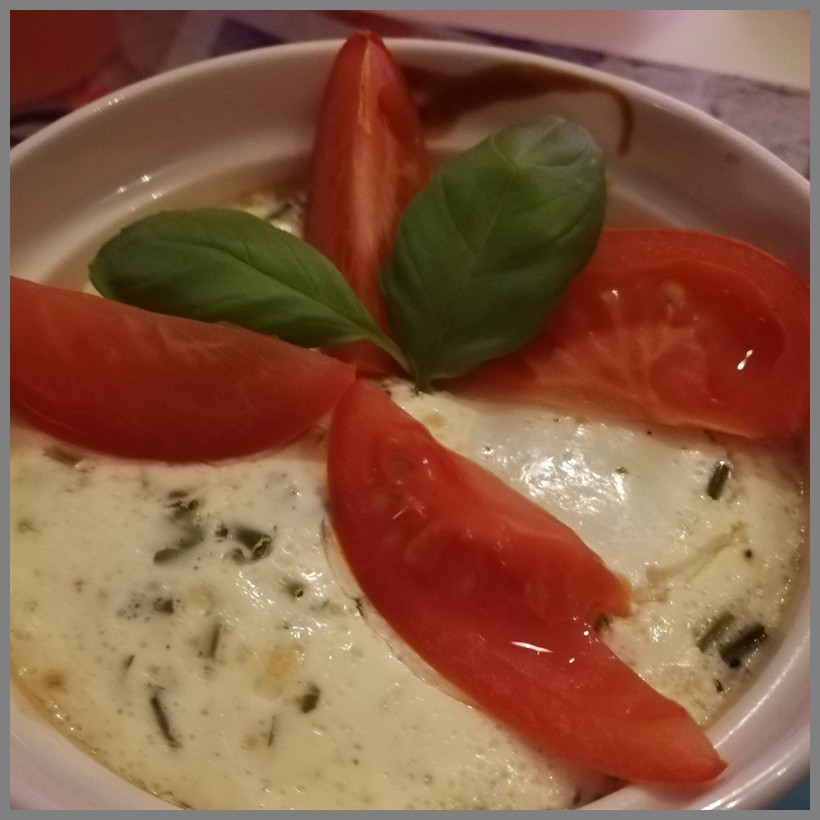
\includegraphics[width=\textwidth]{img/ei_naepfchen_franz.jpg} \cite{eiimnaepfchenfranz}

\subsection*{So geht's:}

\begin{tabular}{p{15cm}}
	\\
  Den Ofen auf 180 Grad vorheizen.\\
  Schmand mit Gewürzen und Kräutern mischen. \\
  Die Masse teilen. Den ersten Teil in 2 Creme-Brulee-Förmchen geben.\\
  Jeweils ein Ei darauf schlagen und die restliche Creme darauf verteilen. \\
  Eine große Auflaufform zur Hälfte mit Wasser füllen. \\
  Die Förmchen hineinstellen und so in den Ofen schieben.\\
  25 Minuten garen lassen.\\
  Circa 5min vor Ende der Zeit zwei geviertelte Tomaten auf den Schälchen verteilen.\\
  Aus dem Ofen holen und auf einem Küchenpapier abtropfen lassen. Brot aufschneiden und servieren.
\end{tabular}

\section{\textsc{Pochiertes Ei in Senfsoße}}

\subsection*{Zutaten:}

\begin{tabular}{p{7.5cm} p{7.5cm}}
	& \\
	100g Butter & 1 Zwiebel \\
	3EL Mehl & 250ml Milch \\
  250ml Gemüsebrühe & 4 Eier \\
  2EL Senf & 5EL Essig \\
  1,5l Wasser &
\end{tabular}

\subsection*{Serviervorschlag:}


\includegraphics[width=\textwidth]{img/ph.jpg} \cite{eisenfsosse}

\subsection*{So geht's:}

\begin{tabular}{p{15cm}}
	\\
  Die Butter in einem Topf zerfließen lassen. Zwiebeln klein würfeln und in die Butter geben.\\
  Glasig anschwitzen lassen. Nach und nach das Mehl darauf verteilen – Mehlschwitze entstehen lassen.\\
  Die Milch dazugeben und kräftig umrühren, damit sich keine Klümpchen bilden.\\
  Die Gemüsebrühe dazu geben. Langsam köcheln lassen.\\
  In einem kleinen Topf das Wasser zum Kochen bringen. Essig hinzufügen.\\
  Die Eier in einer flachen Tasse aufschlagen, ohne das Eigelb zu beschädigen.\\
  Dieses nun schnell, aber mit Bedacht in das kochende Wasser gleiten lassen.\\
  Je nach Geschmack 4-7min pochieren lassen.\\
  Danach die Eier in die Senfsoße geben und nochmals zusammen aufkochen lassen.\\
  Dazu passen hervorragend Petersilienkartoffeln oder luftiges Kartoffelpüree.
\end{tabular}

\section{\textsc{Spaghetti-Spinat-Carbonara mit pochiertem Ei}}

\subsection*{Zutaten:}

\begin{tabular}{p{7.5cm} p{7.5cm}}
	& \\
	200g Spaghetti & 2 Handvoll frischer Blattspinat \\
	\sfrac{1}{2} gewürfelte Zwiebel & \sfrac{1}{2} Knoblauchzehe \\
  40g Bacon & 3 Eier \\
  100ml Sahne & Schuss Essig \\
  Salz, Pfeffer & 1El Sonnenblumenöl
\end{tabular}

\subsection*{Serviervorschlag:}


\includegraphics[width=\textwidth]{img/ph.jpg}

\subsection*{So geht's:}

\begin{tabular}{p{15cm}}
	\\
  Zuerst die Spaghetti nach Packungsanweisung „al denkte“ kochen.\\
  Danach den Bacon in 4cm lange Streifen schneiden.\\
  Das Öl in eine heiße Pfanne geben und die Zwiebeln und Bacon kross anbraten.\\
  Nach etwa 5 Minuten den Spinat dem hinzufügen und so lange mit braten lassen, bis dieser zusammenfällt.\\
  Mit Pfeffer und Salz kräftig würzen.\\
  Nun mit den Spaghetti zusammen in eine größere Pfanne (bzw. Bräter) geben.\\
  Die Sahne in einen Messbecher geben und ein Ei hinzufügen.\\
  Beides verquirlen. Über den Spinatmix geben und alles einreduzieren lassen.\\
  In einem anderen Topf circa 1,5l Wasser zum Kochen bringen.\\
  Hitze runterdrehen, sodass das Wasser nur noch leicht köchelt.\\
  Den Essig dazugeben. Ein Ei in einer flachen Tasse aufschlagen.\\
  Hierbei darauf achten, dass das Eigelb unbeschädigt bleibt.\\
  Von der Tasse, dass Ei langsam in das heiße Wasser gleiten lassen.\\
  6-7 Minuten pochieren lassen. Vorgang mit anderem Ei wiederholen.
\end{tabular}

\section{\textsc{Eierkuchen}}

\subsection*{Zutaten für 2 Portionen:}

\begin{tabular}{p{7.5cm} p{7.5cm}}
	& \\
	100g Mehl & 40g Zucker \\
	300ml Milch & 4 Eier \\
	Prise Salz & Öl für die Pfanne \\
	\multicolumn{2}{l}{Puderzucker zum Dekorieren}
\end{tabular}

\subsection*{Serviervorschlag:}


\includegraphics[width=\textwidth]{img/ph.jpg}

\subsection*{So geht's:}

\begin{tabular}{p{15cm}}
	\\
	Die Eier trennen und das Eiweiß mit einem Schneebesen zu Eischnee schlagen.\\
	Den Zucker, die Milch, das Eigelb und die Prise Salz vermischen.\\
	Das Mehl in die Mischung sieben. Dadurch wir der Teig feiner.\\
	Nun den Eischnee langsam und sorgfältig unterheben, damit es nicht wieder zerfällt.\\
	Das Öl in einer Pfanne erhitzen. Zur Überprüfung die Rückseite eines Holzkochlöffels, oder einen Holzstab ins Öl halten. Schlägt das Öl Blasen, ist es heiß genug.\\
	Den Teig mit einer mittelgroßen Kelle in die Pfanne geben.\\
	Die Pfannkuchen nun auf beiden Seiten goldbraun anbraten.\\
	Mit Puderzucker bestreuen und heiß servieren.
\end{tabular}

\section{\textsc{Pfannkuchen}}

\subsection*{Zutaten für 2 Portionen:}

\begin{tabular}{p{7.5cm} p{7.5cm}}
	& \\
	\sfrac{1}{4}l Milch & 2 Eier \\
	4EL Mehl & Prise Satz \& Zucker \\
  Öl für die Pfanne
\end{tabular}

\subsection*{Serviervorschlag:}


\includegraphics[width=\textwidth]{img/ph.jpg} \cite{pfannkuchen}

\subsection*{So geht's:}

\begin{tabular}{p{15cm}}
	\\
  Öl in der Pfanne heiß werden lassen. In der Zwischenzeit die Zutaten ordentlich vermengen.\\
  Das Mehl sollte keine großen Klümpchen bilden. Wer mag, kann das Mehl auch vorher sieben.\\
  Den Teig mit einer großen Suppenkelle in die Pfanne geben.\\
  Sobald sich der äußere Rand der Pfannkuchen braun färbt, ist es Zeit diese zu wenden. \\
  Auf der anderen Seite auch noch braun werden lassen und servieren.\\
  Mit Puderzucker, oder Zimt bestäuben und fertig.
\end{tabular}


\newpage
\renewcommand{\refname}{\textsc{Bilderverzeichnis}}
\begin{thebibliography}{9}

	\bibitem[Rohkostsalat mit Apfel]{rohkostapfel} Lisa Machoi, 2019
	\bibitem[Amerikanischer Krautsalat]{uskrautsalat} Lisa Machoi, 2019
	\bibitem[Schneller Gurkensalat mit saurer Sahne und Dill]{gurkensalatdill} Lisa Machoi, 2019
	\bibitem[Gurkensalat]{gurkensalat} Lisa Machoi, 2019	
	\bibitem[Frühlingshafter Eiersalat]{fruehlingeiersalat} Lisa Machoi, 2019
	\bibitem[Omelett]{omlett} Lisa Machoi, 2019
	\bibitem[Gewienertes Omelett]{omlettwiener} Lisa Machoi, 2019
	\bibitem[Omelett ToMo]{omlettomo} Lisa Machoi, 2019
	\bibitem[Spiegelei]{spiegelei} Lisa Machoi, 2019
	\bibitem[Spiegelei auf italienisch]{itaspiegelei} Lisa Machoi, 2019
	\bibitem[Rührei]{ruehrei} Lisa Machoi, 2019
	\bibitem[Rührei auf Vollkornbrötchen]{ruehreivollkorn} Lisa Machoi, 2019
	\bibitem[Ei im Näpfchen]{eiimnaepfchen} Lisa Machoi, 2019
	\bibitem[Französisches Ei im Näpfchen]{eiimnaepfchenfranz} Lisa Machoi, 2019
	\bibitem[Pochiertes Ei in Senfsoße]{eisenfsosse} Lisa Machoi, 2019
	\bibitem[Spaghetti-Spinat-Carbonara mit pochiertem Ei]{eicorbonara} Lisa Machoi, 2019
	\bibitem[Eierkuchen]{pancakes} Lisa Machoi, 2019
	\bibitem[Pfannkuchen]{pfannkuchen} Lisa Machoi, 2019

\end{thebibliography}
	\vspace{2cm}
\begin{center}
	Alle \LaTeX - Dokumente verfügbar unter\\ \href{https://github.com/lisamachoi/kochprojekt}{\textbf{https://github.com/lisamachoi/kochprojekt}}
	
	\vspace{2cm}
	
	Dieses Dokument ist lizensiert unter der\\ \href{https://creativecommons.org/licenses/by-sa/4.0/}{\textbf{Creative Commons Attribution-ShareAlike 4.0 International}}\\
	Lizenz.

	\vspace{1cm}

	{\huge\ccbysa}
\end{center}


\end{document}
